\documentclass{article}

\usepackage{amsmath}
\usepackage{amssymb}

\usepackage{minted}

\usemintedstyle{mystyle}

\usepackage[utf8]{inputenc}

\usepackage{pgfplots}

\pgfplotsset{compat=1.16}

\pgfplotsset{every axis/.append style={
	axis lines = left,
	xmin = 0,
	xmax = 10,
	ymin = 0,
	ymax = 10,
	xlabel style = {anchor = west},
	ylabel style = {anchor  =south},
    clip = false,
    ticks = none,
}}

\pgfplotsset{every axis plot/.append style={
	color=black,
	samples=100,
	thick
}}

\definecolor{red}{RGB}{199, 68, 64}
\definecolor{green}{RGB}{64, 199, 70}
\definecolor{blue}{RGB}{45, 111, 177}
\definecolor{yellow}{RGB}{230, 200, 0}
\definecolor{purple}{RGB}{197, 92, 212}

\title{Introduction to \LaTeX}
\author{Onni Olkkonen}
\date{14.4.2025}

\begin{document}

\maketitle

\section{Introduction}

\LaTeX is a language and a tool for creating professionally typeset documents.
Writing plain text is as simple as with any other program.
\textbf{Text} can be \textit{formatted} with \emph{commands}.

\begin{minted}{latex}
	\textbf{Bolded text.}
	\textit{Italisized text.}
	\underline{Underlined text.}
	\emph{Emphasized text}
\end{minted}

\section{Document Structure}

In \LaTeX the document can be divided into sections with the following commands. This document utilizes only sections and subsections. \newline

\begin{tabular}{ c|c|c }
	Command & Level & Comment \\
	\hline
	part & -1 & not in letters \\
	chapter & 0 & only books and letters \\
	section & 1 & not in letters \\
	subsection & 2 & not in letters \\
	subsubsection & 3 & not in letters \\
	paragraph & 4 & not in letters \\
	subparagraph & 5 & not in letters
\end{tabular}

\newpage

\section{Lists}

There are two types of lists: ordered and unordered.

\subsection{Ordered Lists}

Lesson structure
\begin{enumerate}
	\item Introduction
	\item Syntax
	\item Challenge
\end{enumerate}

\begin{minted}{latex}
Lesson structure
\begin{enumerate}
	\item Introduction
	\item Syntax
	\item Challenge
\end{enumerate}
\end{minted}

\subsection{Unordered Lists}

IB subjects
\begin{itemize}
	\item Finnish
	\item English
	\item Mathematics
	\item Economics
	\item History
	\item Chemistry
	\item Physics
	\item Biology
	\item Computer Science
\end{itemize}

\newpage

\begin{minted}{latex}
IB subjects
\begin{itemize}
	\item Finnish
	\item English
	\item Mathematics
	\item Economics
	\item History
	\item Chemistry
	\item Physics
	\item Biology
	\item Computer Science
\end{itemize}
\end{minted}

\section{Math}

In \LaTeX there are essentially two ways of writing mathematics. \textbf{Inline math} is a part of text and \textbf{display math} can be used for more complex equations requiring the whole width of the screen. The Pythagorean theorem ($a^2 + b^2 = c^2$) is one of the most well known pieces of mathematics. Another popular example is the quadratic formula: $s = \frac{-b \pm \sqrt{b^2 - 4 a c}}{2 a}$. However, sometimes math requires more space and display math is needed.

\begin{align*}
& \lim_{ x \to -\infty } \frac{e^{-x}-3e^{-2x}}{e^{-2x}-4} \\
= & \lim_{ x \to -\infty } \frac{e^{-x}-3e^{-2x}}{e^{-2x}-4} \cdot \frac{e^{2x}}{e^{2x}} \\
= & \lim_{ n \to -\infty } \frac{e^{x}-3e^{0}}{e^{0}-4e^{2x}} \\
= & \lim_{ x \to -\infty } \frac{e^{x}-3}{1-4e^{2x}} \\
= & \frac{-3}{1} \\
= & -3
\end{align*}

\begin{minted}{latex}
\begin{align*}
& \lim_{ x \to -\infty } \frac{e^{-x}-3e^{-2x}}{e^{-2x}-4} \\
= & \lim_{ x \to -\infty } \frac{e^{-x}-3e^{-2x}}{e^{-2x}-4} \cdot \frac{e^{2x}}{e^{2x}} \\
= & \lim_{ n \to -\infty } \frac{e^{x}-3e^{0}}{e^{0}-4e^{2x}} \\
= & \lim_{ x \to -\infty } \frac{e^{x}-3}{1-4e^{2x}} \\
= & \frac{-3}{1} \\
= & -3
\end{align*}
\end{minted}

\section{Graphs}

The \textbf{TikZ} package can be used to create graphics.

\subsection{Setup}

\begin{minted}{latex}
\usepackage{pgfplots}

%General style%
\pgfplotsset{every axis/.append style={
	axis lines = left,
	xmin = 0,
	xmax = 10,
	ymin = 0,
	ymax = 10,
	xlabel style = {anchor = west},
	ylabel style = {anchor  =south},
    clip = false,
    ticks = none,
}}

%Functions%
\pgfplotsset{every axis plot/.append style={
	color=black,
	samples=100,
	thick
}}

%Usage%
\begin{document}
...
\begin{tikzpicture}
  \begin{axis}
	...
  \end{axis}
\end{tikzpicture}
...
\end{document}

\end{minted}

\subsection{Lines}

\begin{minted}{latex}
\draw [options] (0,0) -- (10,10);
\end{minted}

\noindent alternatively

\begin{minted}{latex}
\addplot [options] coordinates {(0,0) (10,10)};
\end{minted}

\subsection{Arrows}

\begin{minted}{latex}
\draw [->] (0,0) -- (10,10);
\draw [<-] (0,0) -- (10,10);
\draw [<->] (0,0) -- (10,10);
\end{minted}

\subsection{Polygons}

\begin{minted}{latex}
\fill[options] (0,0) -- (0,10) -- (10,10) -- (10,0) -- (0,0);
\end{minted}

\subsection{Labels}

The location of labels can be specified with coordinates or as relative to some other shape.
Note: \LaTeX can be used in labels.

\subsubsection{Isolated Labels}

\begin{minted}{latex}
\node [left]  at (0,0) {Label};
\node [right] at (0,0) {Label};
\node [above] at (0,0) {Label};
\node [below] at (0,0) {Label};

\node at (0,0) {Label};
\end{minted}

\subsubsection{Relative Labels}

\begin{minted}{latex}
\addplot[] coordinates{(0,0) (10,10)} node[right]{$f$};
\end{minted}

\subsection{Functions}

\begin{minted}{latex}
\addplot[] {x^2};
\end{minted}

\subsection{Example}

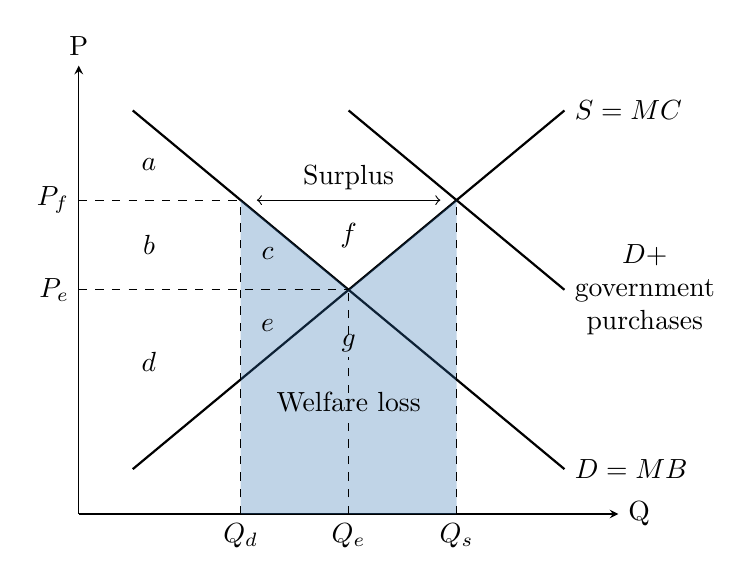
\begin{tikzpicture}
  \begin{axis}
    \node [right] at (current axis.right of origin) {Q};
    \node [above] at (current axis.above origin) {P};
	
    \addplot[] coordinates{(1,9) (9,1)} node[right]{$D=MB$};
    \addplot[] coordinates{(1,1) (9,9)} node[right]{$S=MC$};
    \addplot[] coordinates{(5,9) (9,5)} node[right, align = center]{$D+$ \\ government \\ purchases};
	
    \node [left] at (0,5) {$P_e$};
    \node [left] at (0,7) {$P_f$};
    \node [below] at (3,0) {$Q_d$}; 
    \node [below] at (5,0) {$Q_e$};
    \node [below] at (7,0) {$Q_s$};
	
    \fill[blue, opacity = 0.3] (3,7) -- (5,5) -- (7,7) -- (7,0) -- (3,0) -- (3,7);
	
    \addplot[dashed, thin] coordinates {(0,5) (5,5)};
    \addplot[dashed, thin] coordinates {(5,0) (5,2.2)};
    \addplot[dashed, thin] coordinates {(5,2.7) (5,3.5)};
    \addplot[dashed, thin] coordinates {(5,4) (5,5)};
	
    \addplot[dashed, thin] coordinates {(0,7) (3,7)};
    \addplot[dashed, thin] coordinates {(3,0) (3,7)};
    \addplot[dashed, thin] coordinates {(7,0) (7,7)};
	
    \node at (1.3,7.8) {$a$};
    \node at (1.3,6) {$b$};
    \node at (3.5,5.8) {$c$};
    \node at (1.3,3.4) {$d$};
    \node at (3.5,4.2) {$e$};
    \node at (5,6.2) {$f$};
    \node at (5,3.8) {$g$};
	
    \draw [<->] (3.3,7) -- (6.7,7);
    \node at (5,7.5) {Surplus};
	
    \node at (5,2.5) {Welfare loss};
  \end{axis}
\end{tikzpicture}

\newpage

\begin{minted}{latex}
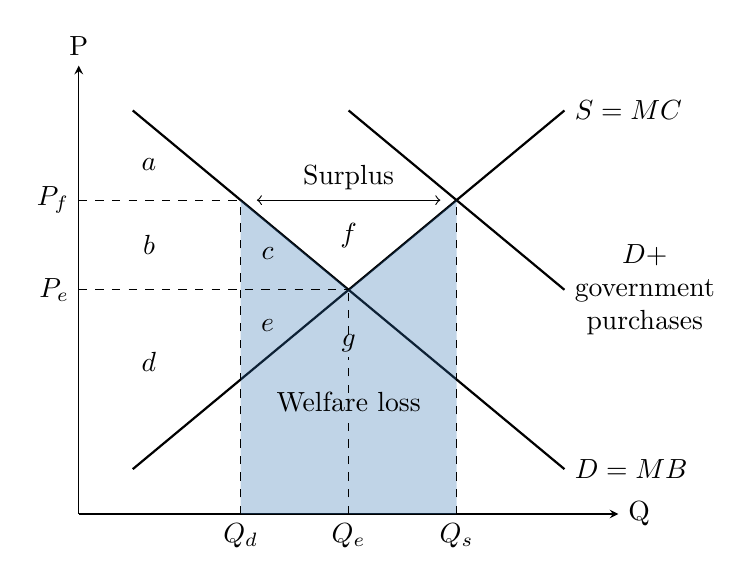
\begin{tikzpicture}
  \begin{axis}
    \node [right] at (current axis.right of origin) {Q};
    \node [above] at (current axis.above origin) {P};
	
    \addplot[] coordinates{(1,9) (9,1)} node[right]{$D=MB$};
    \addplot[] coordinates{(1,1) (9,9)} node[right]{$S=MC$};
    \addplot[] coordinates{(5,9) (9,5)} node[right, align = center]{$D+$ \\ government \\ purchases};
	
    \node [left] at (0,5) {$P_e$};
    \node [left] at (0,7) {$P_f$};
    \node [below] at (3,0) {$Q_d$}; 
    \node [below] at (5,0) {$Q_e$};
    \node [below] at (7,0) {$Q_s$};
	
    \fill[blue, opacity = 0.3] (3,7) -- (5,5) -- (7,7) -- (7,0) -- (3,0) -- (3,7);
	
    \addplot[dashed, thin] coordinates {(0,5) (5,5)};
    \addplot[dashed, thin] coordinates {(5,0) (5,2.2)};
    \addplot[dashed, thin] coordinates {(5,2.7) (5,3.5)};
    \addplot[dashed, thin] coordinates {(5,4) (5,5)};
	
    \addplot[dashed, thin] coordinates {(0,7) (3,7)};
    \addplot[dashed, thin] coordinates {(3,0) (3,7)};
    \addplot[dashed, thin] coordinates {(7,0) (7,7)};
	
    \node at (1.3,7.8) {$a$};
    \node at (1.3,6) {$b$};
    \node at (3.5,5.8) {$c$};
    \node at (1.3,3.4) {$d$};
    \node at (3.5,4.2) {$e$};
    \node at (5,6.2) {$f$};
    \node at (5,3.8) {$g$};
	
    \draw [<->] (3.3,7) -- (6.7,7);
    \node at (5,7.5) {Surplus};
	
    \node at (5,2.5) {Welfare loss};
  \end{axis}
\end{tikzpicture}
\end{minted}

\newpage

\section{Challenge}

\end{document}